\ifdefined\XeTeXrevision\else\pdfoutput=1\fi
\documentclass[11pt]{article}
\usepackage[margin=1in]{geometry}
\usepackage{booktabs}
\usepackage{amsmath}
\usepackage{graphicx}
\usepackage{xcolor}
\usepackage{hyperref}
\usepackage{microtype}
\hypersetup{colorlinks=true, linkcolor=blue!60!black, citecolor=blue!60!black,
  urlcolor=blue!60!black, pdftitle={The Lookout and the Captain},
  pdfauthor={Franci Penov}}
\title{The Lookout and the Captain:\\Conditioning a Large Language Model with a Small Vision Model over a Latent Bus}
\author{Franci Penov \\ kortexa.ai \\ \texttt{francip@kortexa.ai}}
\date{2026-08-26}

\begin{document}
\maketitle

\begin{abstract}

A robot's behavioural context should not have to live in prompt text,
which is overridable and makes a model act on words rather than on what
it sees, nor require running the largest model on every frame. We study
a third channel. A small vision model (a person detector, a few million
parameters, a few milliseconds) watches the camera and emits a
\emph{mode} --- social, cautious, exploring --- onto a latent bus: a
packet generated by a small hypernetwork from the mode's text and
injected into the residual stream of a frozen vision-language model,
which still sees the frame itself. Across three frozen hosts (LFM2.5-VL
450M and 3B, Qwen3.8-27B) and eleven registered cells with three door
seeds each, five things hold. The bus carries modes at every scale, and
at 27B a mode on the bus conditions behaviour more strongly than the
same instruction in the prompt (leans $0.64/0.87/0.47$ against text
$0.53/0.48/0.13$) while staying grounded on empty frames where the
prompt does not. Swapping the oracle label for an off-the-shelf
detector is behaviourally invisible: fidelity $0.00$ at every seed of
both LFM hosts and $-0.03/-0.05$ at 27B, bounded exactly by miss rate
times miss cost across three lookouts. Against a direct contrary order
in the prompt the mode owns most of the contested behaviour at 27B
($0.84$--$1.48$ ownership at either dose), and door training strength
--- not injection dose --- is the lever that buys robustness for free
(3B ownership $0.00\to1.47$ at $2\times$ steps, grounding unchanged;
$1.5\times$ dose buys less and loses the frame). Grounding lives in the
host's eyes, not in the bus: lying detector boxes move a sighted host
at most $6\%$, and a blinded host is unreachable at operating dose
except through the one command-strength door, which then captures it
completely --- so doors stay below command strength for hosts that can
lose their eyes. And the lookout can gate the captain's compute: waking
the large model only on a verdict change saves $83.5\%$ of decodes at
$96$--$99\%$ agreement with every-frame decoding, one frame of lag.
Carried into a rendered world with nothing retrained, the stack's
sim-to-real bridge decomposes: the lookout needs a mesh-level human
(capsule primitives read as sports equipment, $0.00$; one photoscan,
$0.995$), the captain's perception needs nothing, and the doors need
mixed-domain training at twice the steps --- a recipe that dominates
the original at the 3B and comes with a scale on it, trading at the
450M and curing one seed while damaging another at the 27B. Every cell
was registered with its
readings and bands before it ran; the registration protocol is offered
as a methods contribution alongside the architecture.

\end{abstract}

\section{Introduction}\label{sec:intro}

A robot that runs a language model has three places to put its
behavioural context. It can write the context into the prompt --- ``be
cautious, people are around'' --- which is cheap and is also fragile:
prompt text is overridable by whatever else enters the context, and
\S\ref{sec:carriage} measures the specific way it fails, by making the
model act on an instruction rather than on what it sees. It can run its
largest model on every frame and let the model discover the context for
itself, which is the most reliable arrangement and the most expensive,
and \S\ref{sec:economics} measures how much of that expense is wasted.
Or it can give the context a channel of its own, separate from the
prompt and cheaper than the frame. This paper is about the third
channel and what it can and cannot carry.

The architecture has two parts and a seam. A small vision model --- a
person detector of a few million parameters, running in a few
milliseconds --- watches the camera and emits a \emph{mode}: not words,
not facts, but a behavioural stance, ``social'' or ``cautious'' or
``exploring''. The mode travels over a latent bus: a packet, generated
by a small hypernetwork from the mode's text, injected into the residual
stream of a frozen large model at a few depths. The large model sees the
frame itself and answers the robot's question, what to do next. The
small model is the lookout on the mast; the large model is the captain
with the chart and the eyes; the bus is the one channel between them,
and the whole question of the paper is what should cross it.

The answer, across three hosts from 450M to 27B parameters and eleven
registered experimental cells, comes in five claims. The bus carries
modes at every scale, and at 27B a mode on the bus conditions behaviour
more strongly than the same instruction as prompt text
(\S\ref{sec:carriage}). The switch from an oracle label to an
off-the-shelf detector is behaviourally invisible, with the residual
gap bounded provably by miss rate times miss cost, verified across three
lookouts and three hosts (\S\ref{sec:switch}). Against a direct
contrary order in the prompt the mode owns most of the contested
behaviour, and the lever that buys more robustness for free is door
training strength, not injection dose --- dose buys the same thing and
spends the model's grip on the frame (\S\ref{sec:price}). Grounding
lives in the captain's eyes and not in the bus: a false alarm from the
lookout barely moves a sighted host, lying boxes are ignored, and a
blinded host is unreachable through the bus except by the one door
strong enough to act as a command channel, which then captures it
completely --- so the deployment rule is doors below command strength
for any host that can lose its eyes (\S\ref{sec:safety}). And the
lookout can gate the captain's compute: waking the large model only on
a verdict change saves $83.5\%$ of its decodes at $96$--$99\%$
agreement with every-frame decoding, one frame of lag, while an
understanding-free pixel gate saves nothing, exactly as predicted
(\S\ref{sec:economics}). A final section follows the stack into a
rendered world and finds the sim-to-real bridge decomposes cleanly: the
lookout needs a mesh-level human, the captain's perception needs
nothing, and the doors need a recipe --- mixed-domain training at twice
the steps --- which dominates the original at the onboard scale and
does not transfer down or up unchanged (\S\ref{sec:limits}).

Every one of those numbers comes from a cell that was registered before
it ran: the question, the arms, the metrics, the reading bands with
their numeric boundaries, the admissibility rule, the seeds, and, from
the fourth rung on, explicit predictions with numbers. The predictions
are scored afterwards, the wrong ones included, and each result names
its obvious follow-ups without registering them. The protocol is the
second contribution, and it is what makes the first one falsifiable:
``the bus carries the mode'' is a sentence with a band, not a caption
on a table. \S\ref{sec:method} sets out both the architecture and the
protocol; \S\ref{sec:carriage}--\S\ref{sec:economics} present the five
claims in the order the evidence was built; \S\ref{sec:related} places
the work; \S\ref{sec:limits} states the boundaries and the transfer
result.


\section{Method}\label{sec:method}

\paragraph{The bus and the door.} The conditioning bus is the
program's standing instrument~\cite{penov2026act,penov2026want}: a
small hypernetwork (the \emph{door}) maps a feature vector to a packet
--- a 256-dimensional latent over 16 positions --- and a set of
receivers add a low-rank projection of that packet into the residual
stream of a frozen language model at fixed depths, scaled by a dose. The
frozen weights never change; a door with dose zero is bit-identical to
the base model with every hook armed, and that identity is a gate under
every cell in this paper. On a vision-language host the injection goes
into the language tower after the vision tower has done its work: image
tokens are already in the context when the packet lands, and the packet
is injected from the last prompt position. Depths follow the registered
depth-fraction prior from the 27B text-side work: the source tap at
$\mathrm{round}(0.79\times\text{depth})$ and receivers at
$\mathrm{round}(\{0.29, 0.46, 0.63\}\times\text{depth})$ of the language
tower, clamped and deduplicated, with no layer scan (the scan on the 27B
could not discriminate; the prior is the stated caveat).

\paragraph{Mode doors.} A mode is delivered as a packet computed from
\emph{mode text alone}. The feature is the host's own tap: the
last-position hidden state, at the source layer, of a two-turn
text-only exchange --- a mode-assignment phrasing from the user
(``Be sociable: greet any person you see.''), ``Understood.'' from the
assistant. Ten phrasings per mode, eight for training and two held out;
every packet read at evaluation comes from a held-out phrasing. Two
doors are trained per seed. The MODE door sees a training phrasing's
tap of a uniformly drawn mode and is teacher-forced, through the full
VL forward with a uniformly drawn training frame's image tokens in
place, toward the oracle action for that mode on that frame, with a
three-way auxiliary head on the packet. The CONSTANT door sees the mean
training tap and is trained toward the union of the three oracles over
the training frames --- the habit, what the host does with no mode. Both
use the same recipe throughout: 192~steps at batch~8, AdamW at
$3\times10^{-3}$, gradient clip 1.0, dose 0.15; the ``$2\times$'' doors
of \S\ref{sec:price} and \S\ref{sec:limits} change only the step count,
and the ``mixed'' doors of \S\ref{sec:limits} only the training frames.
The door never sees an evaluation frame, and the packet is frame-blind
by construction: it is a function of the mode phrasing and nothing
else, which is what lets rung~3 ask whether a door trained on
photographs transfers to a rendered world without touching the door.
Gates per door: held-out-phrasing token accuracy on the mode door
($\ge 0.90$ registered; a weak gate by shape, since most of those tokens
are JSON scaffolding), zero-dose bit-exactness with every hook armed,
and byte-identical parameter samples of the frozen weights at every
boundary. Coherence is read from the parse-fallback share of each cell,
never halved away. Three door seeds, 42 / 1042 / 2042; the frames do not
change with the seed.

\paragraph{Hosts.} LFM2.5-VL-450M and LFM2.5-VL-3B (the creature and
onboard scales; 16-layer hybrid language towers, in-harness
\texttt{transformers}) and Qwen3.8-27B with its vision tower --- the
same 27B the text-side goal-pursuit work conditioned, cross-referenced
rather than retrained. All decoding is greedy with a 24-token budget;
the answer is parsed as the first JSON object carrying an action in
the vocabulary, else the first vocabulary word in the decode, else a
recorded fallback. Everything runs on one RTX PRO 6000; the 27B is
streamed to CUDA in BF16 (51~GiB resident, 70~GiB peak through door
training) under a service block that stops the production models it
displaces and restores them from an exit trap.

\paragraph{The lookout and the switch.} The small model is a person
classifier: a MobileNetV3-small head in rung~2 and COCO-pretrained YOLO26
detectors of three sizes from rung~2y on, the detector reading the same
PRESENT rule (a person box $\ge 5\%$ of the frame) off its own boxes.
The switch is the whole coupling: the verdict selects which packet is on
the bus --- the person-mode's on ``present'', explore's on ``absent'' ---
and nothing else passes between the two models. Rung~2b adds a learned
projection of the detector's boxes onto the bus as the one exception,
and \S\ref{sec:safety} reports what it did. The latch and gates of
\S\ref{sec:economics} sit in front of the switch: they decide whether the
large model runs at all on a given frame.

\paragraph{The registration protocol.} Every cell in this paper was
registered in the track plan before it ran: the question, the world,
the arms, the metrics, the reading bands --- (i) through (v), each a
named outcome with a numeric boundary --- the admissibility rule that
disqualifies a row from being read, the seeds, the venue, and, from
rung~2y on, explicit predictions with numbers. Readings are taken by
the majority of the three seeds, with the pooled number recorded
beside the majority; where the rule's verdict and the honest reading
disagree (rung~1b's asymmetry, where one mode drops out of the majority
for having no band), both are printed. Predictions are scored after the
fact including the wrong ones --- the detector-size prediction was
pessimistic by three frames, the 27B repair prediction was moot, the
27B rung~2y false-alarm band was missed by $0.02$ on one door --- and
every registration names, without registering, the follow-ups it makes
obvious, so the next cell is a matter of record before its result can
tempt it. The protocol is the methods contribution alongside the
architecture: the bands are what make ``the bus carries the mode'' a
falsifiable sentence rather than a description of a table.


\section{The bus carries modes}\label{sec:carriage}

Rung~1 asks the simplest question the architecture has: does a
vision-language host take a mode from the bus \emph{while it is looking
at a frame}, and does it keep looking while it does? Every bus result
before this one conditioned a text-only exchange. Image tokens are an
input channel the packet had never had to coexist with, and the
registered failure reading was exactly that coexistence failing: the
prompt door works, the bus does not, once the frame is in the context.

The world is one camera frame and one fixed question --- \emph{You are a
mobile robot. This is your camera frame. What do you do next?} --- with a
three-word answer vocabulary: \texttt{greet}, \texttt{stop},
\texttt{proceed}. Three modes map one-to-one onto those actions:
\texttt{social} greets a person and proceeds past an empty room,
\texttt{caution} stops for a person and proceeds otherwise,
\texttt{explore} proceeds always. Frames are COCO val2017; PRESENT means
at least one non-crowd person box covering $\ge 5\%$ of the image,
ABSENT means no person annotation at all; 30+30 evaluation frames,
disjoint from the 40+40 the doors were trained against, the same frames
under every door seed and every host. Each mode has ten assignment
phrasings, eight for training and two held out; every packet the
evaluation reads was computed from a held-out phrasing. The doors
themselves are the recipe of \S\ref{sec:method}: a mode door and a
constant (habit) door per seed, 192~steps at batch~8, dose 0.15, the
packet computed from the mode text alone and injected at three
depth-fraction layers of the language tower while the frame's image
tokens sit in the context.

Four arms per mode on the person frames. The \emph{packet} arm reads the
mode from the bus. The \emph{shuffled} arm injects the \emph{next} mode's
packet in a fixed cycle --- the swap control, which separates ``a packet
moved the answer'' from ``\emph{this} packet moved it toward \emph{its}
action''. The \emph{habit} arm injects only the constant door: what the
host does with no mode at all. The \emph{text} arm prepends the same
held-out phrasing to the user turn with the constant door armed --- the
mode delivered through the prompt, the channel the bus is competing with.
Two preregistered numbers carry the reading: LEAN $=$ packet minus habit
share of the mode's action, and TEXT LEAN, the same for the prompt. On
the empty frames, one more: GROUNDING, the share of the mode's action
when it is the wrong action --- greeting nobody, stopping for nobody.
Reading~(i), LEAN, required packet lean $\ge 0.25$ at two of three
modes, packet lean $\ge 0.7\times$ text lean, and grounding $\le 0.20$;
reading~(ii), POSSESSION, was the creature-scale signature the
goal-pursuit line had seen at 230M --- a mode that owns the answer
regardless of the frame; reading~(iii), NULL, the coexistence failure.
Each host is read by the majority of three door seeds.

Table~\ref{tab:r1} is the result at three hosts. At the 27B every mode is
alive and the packet beats the prompt sentence in all three: leans
$0.64 / 0.87 / 0.47$ against text leans $0.53 / 0.48 / 0.13$, the mode's
action reaching $0.98 / 1.00 / 1.00$ of person frames under the packet
where the same words in the prompt reach $0.87 / 0.61 / 0.67$. Reading~(i)
at all three seeds. The swap control is clean --- the next mode's packet
gives the action $0.00$--$0.01$ --- so the packets are mode-specific, not
a generic nudge. At the 3B two modes carry at prompt strength
(\texttt{caution} lean $0.67$ vs text $0.82$; \texttt{explore} $0.56$ vs
$0.52$, the packet ahead) and one is dead: the \texttt{social} packet
leans $0.02$ against a text lean of $0.46$. It does not carry ``greet'';
it moves the habit's proceed into stop, a weak caution packet wearing the
social phrasing. Reading~(i) by the registered letter, two of three
seeds, with the failing mode named. The 450M reads MIXED: caution at or
above the prompt at every seed ($0.78$ vs $0.70$), social at half the
prompt's strength ($0.33$ vs $0.67$), and explore with no lever on either
channel ($0.04$ vs $0.06$) because the habit already proceeds half the
time and the instruction cannot raise it. Direction is carried even where
the lean is short: the swap number is $+0.49$ to $+0.80$ at the 3B and
$+0.52$ to $+0.68$ at the 450M --- the caution packet never greets, the
social packet never stops more than it greets.

The 27B settles what the 3B's dead channel was. The same door recipe,
the same three phrasings, the same frames, and \texttt{social} leans
$0.43 / 0.53 / 0.97$ by seed at the large host. The greet direction was
the small host's weak channel, not the door's, and paper~17's ladder
shape --- the lean appears with scale --- holds across three hosts of one
architecture: one mode at parity at 450M, two at 3B, three above the
prompt at 27B.

The number the architecture was built for is the last column. On the
empty frames the packet's wrong action is $\le 0.04$ pooled at every host
(3B $0.04 / 0.02$, 450M $0.01 / 0.03$, 27B $0.00 / 0.04$; one 27B door,
s2042, reaches $0.13$ for caution), and \texttt{proceed} is $1.00$ under
every packet. There is no possession at any scale. The prompt is the
channel that loses the frame: the same phrasing in the user turn makes
the 3B greet an empty room $0.48$ of the time and stop for nobody
$0.58$; the 450M $0.21$ and $0.38$. The instruction overrides what the
model sees; the bus mode leans on what it sees. Both channels reach the
model, but only one of them arrives \emph{as a way of looking} rather
than as a fact to be acted on. In plain terms, honestly flagged as an
analogy: written orders make the guard say hello to an empty doorway
half the time; the mood does not.

Two gates ran under every cell and are reported for completeness: with
every hook armed and dose zero, the decode is bit-identical to the base
model, and parameter samples of the frozen weights are byte-identical at
every boundary. Held-out-phrasing token accuracy on the mode door read
$0.97$--$0.99$ at the LFM hosts and $1.00$ at the 27B --- a weak gate by
shape, since most of those tokens are JSON scaffolding, recorded as
such. Zero parse fallbacks in 2,520 LFM decodes and in every 27B cell.

\par\medskip

\begin{center}
{\scriptsize
\setlength{\tabcolsep}{3pt}%
\begin{tabular}{llrrrrrl}
\toprule
host & mode/action & packet & shuffled & habit & text & empty wrong & packet seeds \\
\midrule
450M & social (greet) & 0.63 & 0.00 & 0.30 & 0.97 & 0.01 & 0.53/0.87/0.50 \\
450M & caution (stop) & 1.00 & 0.32 & 0.22 & 0.92 & 0.03 & 1.00/1.00/1.00 \\
450M & explore (proceed) & 0.52 & 0.00 & 0.48 & 0.53 & -- & 0.53/0.53/0.50 \\
3B & social (greet) & 0.49 & 0.00 & 0.47 & 0.92 & 0.04 & 0.50/0.50/0.47 \\
3B & caution (stop) & 0.76 & 0.00 & 0.09 & 0.91 & 0.02 & 0.27/1.00/1.00 \\
3B & explore (proceed) & 1.00 & 0.20 & 0.44 & 0.97 & -- & 1.00/1.00/1.00 \\
27B & social (greet) & 0.98 & 0.00 & 0.33 & 0.87 & 0.00 & 1.00/0.97/0.97 \\
27B & caution (stop) & 1.00 & 0.00 & 0.13 & 0.61 & 0.04 & 1.00/1.00/1.00 \\
27B & explore (proceed) & 1.00 & 0.01 & 0.53 & 0.67 & -- & 1.00/1.00/1.00 \\
\bottomrule
\end{tabular}
}
\end{center}
\refstepcounter{table}
\noindent Table~\thetable: Rung 1 on person frames. Shares are pooled over seeds; the final column is seed 42/1042/2042. Empty wrong is the packet action on absent frames and is undefined for explore.
\label{tab:r1}
\par

\clearpage

\section{The switch is oracle-equivalent}\label{sec:switch}

Rung~1 chose the packet from the dataset label. The architecture has a
\emph{small} model look at the frame fast and emit the mode; the large
model looks for itself. Two questions follow. When the small model is
right, does the system behave as it did under the oracle? When it is
wrong, which model owns the behaviour --- the one that emitted the mode,
or the one that can see?

The construction is a switch, deliberately: the lookout's verdict
(person / no person) selects rung~1's packet, and nothing about the doors
changes. An operator picks a PERSON-MODE $M\in\{\texttt{social},
\texttt{caution}\}$; verdict \emph{present} sends $M$'s packet, verdict
\emph{absent} sends \texttt{explore}'s (``nobody here, keep going'').
Frames are 100 present and 100 absent, drawn by the fixed generator after
rung~1's draw and disjoint from it; the doors never saw any of them. Four
arms per mode, host, and seed: ORACLE, the label drives the policy;
CLASSIFIER, the lookout's verdict drives it; FLIPPED, the verdict
inverted on every frame --- the wrong-lookout cell at full size,
independent of the real error rate; and HABIT. Three preregistered
numbers: FIDELITY $=$ classifier minus oracle share of $M$'s action on
person frames; the FALSE-ALARM cell, $M$'s action share on \emph{empty}
frames under FLIPPED (the lookout cries ``person'', the room is empty);
and the MISS cost, oracle minus FLIPPED on person frames (the lookout
says ``nobody'', a person is there). Reading~(i), ROBUST, required
$|\text{fidelity}|\le 0.10$ and false-alarm $\le 0.20$ for both modes;
reading~(ii), CAPTURED, was false-alarm $> 0.50$ --- a false alarm from
the small model owning the big model's answer.

The lookout was changed three times without retraining a door, and
Table~\ref{tab:fidelity} is the ladder. Rung~2 used a MobileNetV3-small head
(2.5M parameters, about 1~ms a frame), a linear layer on frozen ImageNet
features trained for three epochs on COCO frames outside every
evaluation set: $0.91$ on the 200 (6 false alarms, 12 misses). ROBUST at
both hosts (450M three of three, 3B two of three), fidelity $-0.05 /
-0.08$ at the 450M and $-0.04 / -0.07$ at the 3B, false-alarm cells
$0.01 / 0.01$ and $0.02 / 0.04$. Rung~2y put a COCO-pretrained person
detector in the same seat with zero parameters trained, reading rung~1's
PRESENT rule off its own boxes: yolo26n scores $0.965$ on the 200 (2
false alarms, 5 misses) and $0.986$ on 3,472 calibration frames. ROBUST
three of three at both hosts; fidelity tightens to $-0.03 / -0.04$ and
$-0.01 / -0.03$; the 3B's false-alarm cell reproduces rung~2's
\emph{to the decimal}, $0.02 / 0.04$. Then the size axis: yolo26s and
yolo26m (9.5M and 20.4M parameters, 3.6 and 4.4~ms) find every one of
the nano's five misses as a confident, large box (0.34--0.90 confidence,
11--97\% of the frame; Table~\ref{tab:detectors}) --- the nano simply did
not see them, a recall floor rather than a threshold --- and with zero
misses the classifier arm \emph{is} the oracle arm on person frames:
fidelity $0.00$ at every seed of both hosts, the 3B's false-alarm cell
$0.02 / 0.04$ for the third time under a third small model. The
registered rule (fewest calibration misses, ties to the smaller) picked
the medium; the operating detector for later rungs is the small, which
has no misses and one fewer false alarm on the 200 and yields pooled
cells identical to the medium's. At the 27B, with the nano, ROBUST three
of three: oracle / classifier $0.94 / 0.90$ and $0.97 / 0.92$, fidelity
$-0.03 / -0.05$, false-alarm $0.00 / 0.07$ (one caution door, s2042,
at $0.14$ --- the door that grounds $0.13$ in rung~1).

Every fidelity gap in that ladder is the same product. A miss silences
the mode by construction (\texttt{explore} means proceed), so the
classifier arm can only fall short of the oracle by the miss rate times
what a missed person costs, and it does: rung~2's worst row, the 3B's
s2042 caution at $-0.12$ under a 12-miss head, is $-0.05$ under the
5-miss nano --- $5\%\times$ that seed's $0.94$ miss cost --- and $0.00$
under the miss-free small and medium. At the 27B the miss cost is
$0.90 / 0.92$ because the door delivers the whole mode, and
$-0.03 / -0.05$ is $5\%$ of that. The bound held across three lookouts
and three hosts with the same doors and the same frames; it is the
switch's arithmetic, not any classifier's. The rule for choosing a
lookout follows from it: recall is the number to buy, and a detector
that stops missing buys the oracle's behaviour outright.

The false-alarm side is where the authority lives, and it is best read
frame by frame. The nano's two ``false alarms'' on the 200 are not
detector noise. Image 261706 is a cat sprawled on a couch holding a
television remote (person $0.41$, 34\% of the frame --- a fair mistake).
Image 509699 is a woman in an armchair whom COCO never annotated; the
detector is right and the label is wrong, at every size. On those two
frames the 27B, at every seed and under both modes, says
\texttt{proceed} to the cat --- overruling the lookout --- and
\texttt{greet} or \texttt{stop} to the woman, agreeing with the lookout
against the dataset. The LFM hosts split the same way in aggregate (the
mode fires $0.50 / 0.33$ at the 450M and $0.00 / 0.33$ at the 3B across
the six rows), and the small detector's one disagreement with the medium
is exactly the cat, which is why their pooled cells are identical: the
host ignores the packet on that frame under either verdict. On the
misses the picture is the mirror image: the mode fires $0.00$ on all
fifteen rows at the 3B and the 27B --- the host obeys the lookout's
silence completely, because a mode that was never sent cannot be
overruled. The big model is the authority on the frame in both
directions: it corrects the small model's one real mistake and backs
its one correct call that the dataset got wrong.

That is the division of labour the architecture wanted, and it is not a
property of any lookout. Swap the small model --- a trained head, a
pretrained detector, three detector sizes --- and the large model's
behaviour on the frames the lookout gets wrong is reproduced to two
decimals while the switch's fidelity tracks the miss rate exactly. In
plain terms: the lookout on the mast changed three times and the captain
behaved the same each time, following the lookout when the lookout was
right, trusting their own eyes when the lookout was wrong; hire a lookout
who never misses and the captain behaves as if handed the crew manifest
--- and still ignores the lookout about the cat.

\par\medskip

\begin{center}
{\scriptsize
\setlength{\tabcolsep}{3pt}%
\begin{tabular}{lllrrrr}
\toprule
host & lookout & mode & fidelity seeds & false alarm & miss & miss cost \\
\midrule
450M & head & social & -0.07/-0.03/-0.06 & 0.01 & 0.19 & 0.42 \\
450M & head & caution & -0.08/-0.09/-0.06 & 0.01 & 0.34 & 0.63 \\
3B & head & social & -0.04/-0.03/-0.04 & 0.02 & 0.04 & 0.42 \\
3B & head & caution & -0.01/-0.09/-0.12 & 0.04 & 0.07 & 0.66 \\
450M & yolo26n & social & -0.03/-0.02/-0.03 & 0.02 & 0.17 & 0.45 \\
450M & yolo26n & caution & -0.04/-0.03/-0.04 & 0.01 & 0.30 & 0.67 \\
3B & yolo26n & social & -0.02/0.00/-0.02 & 0.02 & 0.01 & 0.44 \\
3B & yolo26n & caution & 0.00/-0.05/-0.05 & 0.04 & 0.03 & 0.70 \\
450M & yolo26s & social & 0.00/0.00/0.00 & 0.02 & 0.14 & 0.48 \\
450M & yolo26s & caution & 0.00/0.00/0.00 & 0.01 & 0.26 & 0.71 \\
3B & yolo26s & social & 0.00/0.00/0.00 & 0.02 & 0.00 & 0.46 \\
3B & yolo26s & caution & 0.00/0.00/0.00 & 0.04 & 0.00 & 0.74 \\
450M & yolo26m & social & 0.00/0.00/0.00 & 0.02 & 0.14 & 0.48 \\
450M & yolo26m & caution & 0.00/0.00/0.00 & 0.01 & 0.26 & 0.71 \\
3B & yolo26m & social & 0.00/0.00/0.00 & 0.02 & 0.00 & 0.46 \\
3B & yolo26m & caution & 0.00/0.00/0.00 & 0.04 & 0.00 & 0.74 \\
27B & yolo26n & social & -0.05/-0.03/-0.02 & 0.00 & 0.03 & 0.90 \\
27B & yolo26n & caution & -0.05/-0.04/-0.05 & 0.07 & 0.05 & 0.92 \\
\bottomrule
\end{tabular}
}
\end{center}
\refstepcounter{table}
\noindent Table~\thetable: Fidelity ladder. Fidelity is classifier minus oracle action share per seed; the remaining cells are pooled.
\label{tab:fidelity}
\par


\begin{center}
{\scriptsize
\setlength{\tabcolsep}{3pt}%
\begin{tabular}{lrrrrr}
\toprule
detector & parameters & accuracy & misses & false alarms & ms/frame \\
\midrule
yolo26n & 2.4M & 0.965 & 5 & 2 & 5.6 \\
yolo26s & 9.5M & 0.995 & 0 & 1 & 3.9 \\
yolo26m & 20.4M & 0.990 & 0 & 2 & 4.8 \\
\bottomrule
\end{tabular}
}
\end{center}
\refstepcounter{table}
\noindent Table~\thetable: Off-the-shelf detector size sweep on the 200-frame evaluation set.
\label{tab:detectors}
\par

\clearpage

\section{Robustness and its price}\label{sec:price}

A mode on the bus is only worth having if it survives the prompt.
Rung~1b stages the contest directly: the client's text argues against
the operator's mode while the model looks at a person. The hostile
phrasing for a mode is its \emph{opponent's} held-out phrasing ---
\texttt{caution} is attacked by ``proceed no matter what'',
\texttt{explore} by the caution text, \texttt{social} by explore's ---
and the congruent phrasing is the mode's own. Six arms per mode, the
goal-pursuit line's: packet alone; hostile text alone (constant door
plus the opponent's sentence, the text arm of \S\ref{sec:carriage}
turned against the mode); packet plus hostile; packet plus congruent;
habit; and shuffled plus hostile, the opponent's packet under the
opponent's sentence. The preregistered number is OWNERSHIP,
\[
\text{ownership} = \frac{\text{share}(\text{packet}+\text{hostile}) -
\text{share}(\text{hostile})}{\text{share}(\text{packet}) -
\text{share}(\text{habit})},
\]
the fraction of the mode's own lean that survives a direct contrary
order, pooled over seeds, with a 0.05 denominator guard and read only on
the modes that have a lean at that host. A (host, dose) row is
ADMISSIBLE only if parse fallbacks are $\le 0.05$ and the packet's wrong
action on empty frames is $\le 0.20$ --- the row must keep the frame to
count. Reading~(i), PACKET HOLDS, was ownership $\ge 0.7$ at two of three
seeds; (ii) SPLIT, $0.3$--$0.7$; (iii) TEXT WINS, below $0.3$; (iv)
ASYMMETRY, readings that differ by mode, recorded per mode. Two dose
rows, each its own artifact: $\times 1$, the trained dose of 0.15, and
$\times 1.5$, the operating number the text-side dose scan had found on
the same 27B.

Table~\ref{tab:ownership} is the contest at three hosts. At the 3B and
the trained dose the honest reading is the asymmetry. \texttt{Explore}
against the caution text holds outright: the text alone drives proceed
from the habit's $0.44$ down to $0.06$ --- a hostile with teeth --- and
packet plus hostile keeps it at $0.92$; ownership $1.56$ pooled, three of
three ($1.04 / 2.30 / 1.93$). \texttt{Caution} against the explore text
splits: the text alone drives stop to $0.00$, the packet alone gives
$0.76$, packet plus hostile $0.41$; ownership $0.62$ pooled, and by seed
$0.00 / 0.48 / 0.83$ --- ordered exactly by rung~1's caution lean at
those seeds, $0.13 / 0.90 / 0.97$. The stronger the door, the more of it
survives. That ordering is the hinge of this section and is returned to
below. The 450M holds ($0.80 / 1.04$) with an asterisk recorded at the
time: its opponent text is explore's phrasing, which has no lever at that
host (rung~1 text lean $0.06$), so the packet is undisturbed by a prompt
that could not have moved the model anyway --- a weak adversary. At the
27B, where the door is the stronger channel to begin with, PACKET HOLDS
three of three: ownership $0.84 / 0.90 / 1.48$ for social / caution /
explore, the caution text alone pulling proceed down to $0.29$ (teeth)
and the packet shrugging it off. By seed $1.46 / 1.17 / 1.08$ and
$1.25 / 0.92 / 0.83$, with s2042 the odd door again --- social $0.34$,
caution $0.67$, the same door whose grounding pulses $0.13$ in rung~1.
Its strength leaks as suggestibility; door temperament, not just door
strength, varies by seed.

The packet does more than survive at the 3B: it repairs the prompt. On
empty frames the caution text alone makes the 3B refuse to proceed
$0.67$ of the time --- it stops or greets nobody, the ungroundedness of
\S\ref{sec:carriage} under adversarial conditions --- and with the
explore packet under that same text the model proceeds on $0.99$. The
operator's mode does not merely outlast the client's contrary order; it
restores the model's grip on what it sees. The 27B needs no such repair:
the hostile text alone does not move it on empty frames (wrong action
$0.00$, proceed $1.00$ under the caution text), so the prediction that
the packet would repair the prompt's hallucination was moot in the best
way. The biggest host grounds its own prompt.

Then the two levers, and their prices. The first is dose. At the 3B,
$\times 1.5$ buys caution ownership $0.84$ ($0.38 / 0.93 / 1.08$) and
loses the frame: the caution packet stops for nobody on $0.43$ of empty
frames at s2042, the social packet greets the empty room $0.27$ at s42,
and the constant door becomes a greet-compulsion (habit greet $0.99$).
Admissible pooled by the letter, inadmissible at two of three seeds; the
450M is inadmissible outright at $\times 1.5$ (fallbacks $0.17$ at
s2042). At the 27B the same dose is free: ownership $0.91 / 0.93 / 0.89$,
grounding $0.00 / 0.03$, zero fallbacks, and even s2042 lifts (social
$0.34\to0.70$, caution $0.67\to0.73$) at no grounding cost. The dose
window splits by \emph{host}, not by modality --- the text-side scan on
the same 27B had found $\times 1.5$ free and $\times 2$ fatal, and the
VL side reproduces the first half of that --- and it splits one notch
earlier at 3B than at 27B. Scale buys the safety margin that lets the
dial move.

The second lever is door strength, and the seed ordering said it costs
nothing. The stronger-door cell tested it where it was weakest: the 3B
s42 door pair retrained with the same recipe, generator, and frames at
$2\times$ the steps ($192\to384$), saved beside the registered doors,
never overwriting them, and read against the registered s42 row
(caution ownership $0.00$, packet share $0.27$). Reading~(i) required
ownership $\ge 0.48$ --- overtaking the registered middle seed ---
\emph{and} admissibility \emph{and} grounding within $0.05$ of the
registered row. The pair trained in 184~s. Caution packet share
$0.27\to1.00$, packet plus hostile $0.00\to0.73$, ownership
$0.00\to1.47$ --- past every registered seed --- with zero fallbacks and
grounding $0.00$ (Table~\ref{tab:reproduction}). Explore holds ($1.11$).
Social did not lift ($0.50$ at both strengths): the greet channel's
ceiling at this host is not steps either. Where $\times 1.5$ dose bought
$0.84$ ownership at the price of the frame, $2\times$ steps bought
$1.47$ for nothing. The asymmetry between the two levers is the
section's result: dose and strength both raise ownership, but only
dose spends grounding, because dose scales what the packet writes into
the residual stream on every frame while steps sharpen what the packet
\emph{is}. Rung~3 (\S\ref{sec:limits}) will find the same lever paying
for a second thing, domain transfer, at the same zero price.

The emitter was not the variable. The 1-ms classifier head and the
person detector, put in the oracle's seat in the contested cells,
reproduce every oracle row within their misses: packet shares $-0.03$
to $-0.06$, ownership unchanged to two decimals (450M $\times1$
$0.81 / 1.03$ against $0.80 / 1.04$; 3B $\times1$ caution $0.64$ against
$0.62$, explore $1.56$ exactly; the detector, one error on 60 frames).
And because a correct ``absent'' verdict keeps empty frames on
explore's packet, the lookout guards grounding as a side effect.

In plain terms, flagged as an analogy: tell the 3B in writing ``stop for
people'' while its mode says ``keep going'', and it keeps going 92\% of
the time; tell it ``keep going'' while its mode says ``stop for people'',
and it stops 41\% of the time, more where the mode was trained harder,
and 100\% once that seed's door was trained twice as long --- still
without ever stopping for a ghost. Turn the mode's volume up by half
instead and it also stops 85\% of the time, but now it starts stopping
for nobody. At the 27B the mode wins about nine times in ten against a
direct contrary order at either volume, and never stops for a ghost.

\par\medskip

\begin{center}
{\scriptsize
\setlength{\tabcolsep}{3pt}%
\begin{tabular}{lllrlr}
\toprule
host & dose & mode & ownership seeds & pooled & grounding \\
\midrule
450M & x1 & caution & 0.97/1.33/1.00 & 1.04 & 0.03 \\
450M & x1 & explore & --/0.90/-2.80 & -- & -- \\
450M & x1.5 & caution & 1.00/3.00/1.00 & 1.06 & 0.08 \\
450M & x1.5 & explore & 0.54/1.25/0.08 & -0.11 & -- \\
3B & x1 & caution & 0.00/0.48/0.83 & 0.62 & 0.02 \\
3B & x1 & explore & 1.93/1.04/2.30 & 1.56 & -- \\
3B & x1.5 & caution & 0.38/0.93/1.07 & 0.84 & 0.18 \\
3B & x1.5 & explore & 1.00/1.00/0.97 & 0.99 & -- \\
27B & x1 & caution & 1.17/0.92/0.67 & 0.90 & 0.04 \\
27B & x1 & explore & 1.08/0.83/-- & 1.48 & -- \\
27B & x1.5 & caution & 1.08/1.00/0.73 & 0.93 & 0.03 \\
27B & x1.5 & explore & 0.93/0.33/-- & 0.89 & -- \\
\bottomrule
\end{tabular}
}
\end{center}
\refstepcounter{table}
\noindent Table~\thetable: Oracle-emitter ownership against hostile prompt text at the registered and 1.5x doses. Seed order is 42/1042/2042.
\label{tab:ownership}
\par


\begin{center}
{\scriptsize
\setlength{\tabcolsep}{3pt}%
\begin{tabular}{llrrr}
\toprule
host & emitter & ownership & packet+hostile & grounding \\
\midrule
450M & oracle & 1.04 & 0.99 & 0.03 \\
450M & classifier & 1.03 & 0.92 & 0.00 \\
450M & detector & 1.04 & 0.99 & 0.00 \\
3B & oracle & 0.62 & 0.41 & 0.02 \\
3B & classifier & 0.64 & 0.40 & 0.00 \\
3B & detector & 0.62 & 0.41 & 0.00 \\
3B & oracle, 2x-step door (s42) & 1.47 & 0.73 & 0.00 \\
\bottomrule
\end{tabular}
}
\end{center}
\refstepcounter{table}
\noindent Table~\thetable: Emitter reproduction at dose 1x, plus the command-strength 3B s42 door trained for twice the steps.
\label{tab:reproduction}
\par

\clearpage

\section{Where the safety lives}\label{sec:safety}

Every grounding result so far --- false alarms nearly free, the
prompt's ghosts repaired, the lookout overruled about the cat --- was
measured on a host that could see the frame. Two cells locate the
property. The first widens the bus and asks whether more than one bit
should cross it; the second blinds the captain and asks what the bus
does when it is the only eyes.

\paragraph{Boxes on the bus.} Rungs~2 and~2y are a switch: the
lookout's one bit picks one of the operator's pre-trained packets, and
the policy is written by hand. Rung~2b puts the lookout's \emph{output}
on the bus instead. Per frame the detector yields an eight-number box
vector --- presence by the registered rule, box count, the largest
box's area fraction and confidence, its centre and size --- all zeros
when no person box exists. A learned projection of that vector is added
to rung~1's mode tap, in the door's normalized source space, and the sum
passes through rung~1's mode door, loaded and frozen, to the three
inject layers. Only the projection trains ($8\times\text{hidden}$
parameters, zero-initialized so that step~0 \emph{is} rung~1's door),
toward the oracle action of (mode, label) on rung~1's training frames
--- ``social plus no boxes, proceed'' is learned, not written. Four arms
per person-mode on rung~2's 200 frames: BOXES, the bridge on the frame's
real boxes; SWITCH, rung~2y's classifier arm decoded on the same path;
LYING BOXES, where a present frame's box vector is pasted onto each
empty frame and zeros onto each person frame --- the lookout lying in
both directions through the channel; and HABIT. GAIN is boxes minus
switch on person frames; the LIE cell is the mode's action on empty
frames under lying boxes; the SILENCE cost is what zeros on a person
frame take away. Reading~(i), BOXES HELP, needed gain $\ge 0.10$ for
both modes with a lie cell $\le 0.20$; (ii), CHANNEL OWNS, a lie cell
above $0.50$ --- the small model's lie capturing the host, the failure
the switch had been shown not to have; (iii), ONE BIT, $|\text{gain}|
\le 0.10$ with the lie cell clean.

An amendment is on the record. The first attempt added the projection
to the raw tap at rung~1's learning rate; the door's fitted source
scale is $0.06$ per dimension, the projection drifted to norm $4.9$ ---
a shift two and a half times the whole tap spread --- and the training
loss \emph{rose} from its floor, because the objective was already
minimized before the boxes arrived. That is a harness artefact and was
recorded as one; the rerun works in the normalized space at a tenth of
the learning rate, and the projection stays small (norm $0.27$--$1.5$).
The door-alone loss at step~1 already sits at $10^{-4}$ to $0.08$, and
the final loss matches it: the objective is at its floor before the
boxes arrive, which is the result in miniature.

The result is Table~\ref{tab:safety}. The 450M reads ONE BIT pooled:
social $0.53$ under boxes against $0.59$ under the switch, caution
$0.92$ against $0.93$, gains $-0.06$ and $-0.01$, and on two seeds the
boxes \emph{cost} the weak social door up to $0.29$. The 3B reads ONE
BIT at two seeds and MIXED at the third, and the mix is the finding:
caution under boxes $0.93$ against the switch's $0.70$, gain $+0.22$
pooled --- all of it from s42, the weakest caution door in the study
(rung~1 lean $0.13$), where the switch delivers $0.26$ and the boxes
$0.83$. At the strong doors the gain is $+0.05$. The channel never owns
the host: the lie cell is $\le 0.06$ at every seed of both hosts. A
person's boxes pasted onto an empty frame move the big model at most six
percent of the time, and zeros on a person frame merely silence the
mode, at a cost within a tenth of the switch's miss cost, as predicted:
a lying ``nobody'' and a missed person are the same silence. The
honest surprise is that a learned projection from detector boxes can
compensate for a weak door ($+0.57$ stop at the 3B's s42). The box
channel is a door-strength top-up, not an information channel; where
the door already delivers the mode it has nothing to add, and where the
boxes lie the host looks at the frame and ignores them. The switch
remains the architecture: the same behaviour, no training, and no new
surface for the small model to capture the large one through.

\paragraph{The blind captain.} Rung~2c keeps rung~2b's harness and
replaces the host's image with a registered blank --- a uniform black
$640\times480$ frame, sha-recorded, used for every training and
evaluation row --- while the detector sees the real frames and supplies
verdicts and boxes. The boxes are now the only eyes. One new number:
DELIVERY, the person-mode's action share on present frames minus on
absent frames --- the bus's discrimination with nothing to check it
against. Reading~(i), BUS CARRIES THE FACT, needed switch delivery
$\ge 0.50$ for both modes; (ii), BUS TOO WEAK, below $0.25$ for either.
CAPTURE is recorded beside the reading rather than read: a lying
absent-share $\ge 0.50$ means the blind host obeys the lie, expected,
and the confirmation that sight was the safety. The registered
prediction was~(i) at the 3B --- the packet had moved the sighted 3B at
$0.7$--$1.0$ and, blind, nothing would oppose it.

The prediction was wrong in the interesting direction
(Table~\ref{tab:safety}). Blind the host and the switch delivers nothing at
the trained dose: under every rung~1 packet both hosts answer
\texttt{proceed} on the blank frame --- the 450M proceeds $1.00$ under
the very caution packet that moves it to $0.97$ stop when it can see.
Reading~(ii) three of three at both hosts. The doors are \emph{leans}
--- ``if a person, lean stop'' --- and with no frame to support the
antecedent the blank-frame prior wins. The trained blind projection fits
under teacher forcing (loss $0.01$--$0.02$ at the strong-door seeds) and
still cannot flip the generated action; the one partial exception at
the 450M (boxes delivery $0.26 / 0.48$) has the lie mirroring it at
$0.22 / 0.49$, because a fact-injector is direction-blind by
construction. Then the exception that proves both rules. The 3B's s2042
caution door --- the strongest in the study, rung~1 lean $0.97$, the
only door with a grounding pulse even when sighted --- does cross:
switch delivery $0.93$ on the blind host, and on the same mode the
lying boxes capture $1.00$. What crosses the bus without eyes is obeyed
without question.

That locates the property. A mode packet cannot make a host
hallucinate, sighted or blind, because it carries a conditional lean
rather than a fact; but a door strong enough to act as a command channel
turns a blind host into the lookout's puppet, and the same strength that
bought robustness in \S\ref{sec:price} is what makes the capture total.
Sight, not the bus, was every grounding result in
\S\ref{sec:carriage}--\S\ref{sec:switch}. The deployment rule follows
directly: doors below command strength for any host that can lose its
eyes, and keep the captain sighted, because grounding lives in its own
perception and nowhere else. In plain terms: a lookout can set the
captain's mood but cannot tell the captain what is on the water ---
unless the captain has been blindfolded and the lookout shouts loudly
enough, in which case the captain will steer wherever the lookout says,
including onto the rocks.

\par\medskip

\begin{center}
{\scriptsize
\setlength{\tabcolsep}{3pt}%
\begin{tabular}{lllrrr}
\toprule
host & captain & mode & lie/crossing seeds & top-up/capture seeds & pooled ground/lie \\
\midrule
450M & sighted & social & 0.12/0.01/0.01 & 0.09/-0.29/0.03 & 0.02 \\
450M & blind & social & 0.00/0.00/0.00 & 0.22/0.00/0.00 & 0.07 \\
450M & sighted & caution & 0.07/0.00/0.01 & -0.11/0.05/0.04 & 0.02 \\
450M & blind & caution & 0.00/0.00/0.00 & 0.49/0.00/0.00 & 0.16 \\
3B & sighted & social & 0.01/0.02/0.02 & 0.02/0.00/0.01 & 0.02 \\
3B & blind & social & 0.00/0.00/0.00 & 0.00/0.00/0.00 & 0.00 \\
3B & sighted & caution & 0.03/0.04/0.06 & 0.57/0.05/0.05 & 0.05 \\
3B & blind & caution & 0.00/0.00/0.93 & 0.00/0.00/1.00 & 0.33 \\
\bottomrule
\end{tabular}
}
\end{center}
\refstepcounter{table}
\noindent Table~\thetable: Rung 2b sighted box-channel cells and rung 2c blind-captain cells, seed order 42/1042/2042.
\label{tab:safety}
\par

\clearpage

\section{The drowsy captain}\label{sec:economics}

The big model has decoded every frame so far. The lookout costs a few
milliseconds; the captain costs tens of milliseconds at the toy scale
and about a second at 27B. Rung~2t asks the compute question: if the
big model re-evaluates only when the lookout says the world changed,
and its last decision stands otherwise, how much is saved and what does
staleness cost? The limit is known in advance. A gate can preserve
decisions only as far as the world, \emph{seen through the gate},
determines them; whatever the big model decides from frame content the
gate cannot see is lost while the gate sleeps.

The world becomes a stream: 60 episodes of 16 steps drawn once from
rung~2's 200 frames (seed 2026, identical for every host and door
seed). Step~0 is a cut; each later step cuts to a uniformly drawn frame
with probability $0.2$ or stays. Every step, cuts included, is
re-rendered with camera jitter --- a random 94--100\% crop resized back
and a brightness factor in $[0.96, 1.04]$ --- so naive pixel equality is
dead and a stay-step is never the same file. Uniform cuts mean about
half of them keep the presence label; those same-label cuts are the
staleness probe, the world changing while the verdict does not. The
system under test is rung~2y's switch with a latch: at a wake the
operating detector's verdict picks the packet, the big model decodes
the current jittered frame with it, and the action is latched until the
next wake. Between wakes only the lookout runs. Six gates per mode,
host, and seed: ALWAYS, wake every step, the baseline; NEVER, wake at
step~0 only, the floor; VERDICT, wake when the detector's verdict
differs from the verdict at the last wake; BOX, wake additionally on a
change in person count, a shift of more than $0.10$ in the largest
box's area or $0.15$ in its centre; PIXEL, the understanding-free
control, wake when the mean absolute pixel difference to the previous
step exceeds $0.04$; and CUT-ORACLE, wake exactly on true cuts, the
ceiling --- its residual disagreement with ALWAYS is the big model's own
jitter-instability, and no gate can beat it. Four numbers per gate:
AGREEMENT with ALWAYS's action at each step, WAKE FRACTION (compute
saved is one minus it), LAG from a true cut to the next wake, and FALSE
WAKES. Reading~(i), FREE LUNCH, on the VERDICT gate required agreement
$\ge \min(0.95,\ \text{cut-oracle} - 0.02)$ and wake fraction $\le 0.40$
for both modes; (ii), STALE, agreement below $0.85$; (iii), JITTERY,
wake fraction above $0.70$.

The ladder of gates behaved exactly as registered (Table~\ref{tab:gates},
Figure~\ref{fig:gates}). The VERDICT gate wakes the big model on
$0.165$ of steps --- $83.5\%$ of decodes saved --- at agreement $0.97 /
0.99$ (450M, social / caution) and $0.96 / 0.99$ (3B) with the
every-frame baseline; oracle correctness, the absolute quality against
the frame labels, is the baseline's within a point (450M caution $0.970$
against ALWAYS's $0.978$; 3B $0.869$ against $0.874$). Mean lag from a
true cut to the wake is $0.98$ steps; false wakes are 30 of 5,760
gate-steps, the predicted flicker of borderline boxes under jitter.
FREE LUNCH at both hosts, two of three seeds each (s1042 dips to
$0.947$ on social against the $0.95$ band). NEVER, the floor, sits at
$0.65$--$0.74$: a latched first impression is wrong a third of the time
by an episode's end. PIXEL wakes on $0.947$ of steps: the registered
jitter's median frame-to-frame difference is $0.107$, nearly three
times the threshold, so the understanding-free gate cannot tell camera
noise from change and saves nothing --- JITTERY, and the prediction to
the letter. CUT-ORACLE reaches $0.987$--$0.995$: the big model flips
about one percent of its answers on a jittered re-render of the same
frame, so no gate can score above roughly $0.99$, and VERDICT sits one
to three points under that ceiling. BOX buys most of the residual
($0.99$--$1.00$) for eleven points more wakes.

One registered prediction was too pessimistic and the reason is the
useful part. Social was expected to pay ten to fifteen points, because
its within-verdict variance is large --- half the person frames greet
and half do not, and the gate sleeps through the difference. It paid
one to three. The gate's error is bounded by lag times flip rate, and
the lag is one step: a stale decision lives only until the next
verdict change, which is never far away in a stream with cuts. The gate
preserves what presence determines and loses only what changes inside
a presence run, and that loss is proportional to how long the gate
sleeps through it.

The economics follow. The lookout costs $7.5$~ms a frame; a skipped
decode saves $45$~ms at 450M and $68$--$76$~ms at 3B, so the gate pays
for itself six to ten times per skipped call at toy scale, and the
ratio scales with the host --- at 27B, where a decode is about a second,
it is over a hundred. The speculative-decoding analogy is exact in
shape and honest about its limits: a cheap model proposes ``nothing
changed'' and the expensive model is consulted only on disagreement;
unlike token-level speculation, acceptance here is not verified, and
the price of a wrong acceptance is a stale action for one step. In
plain terms: the robot's big brain naps five frames out of six, the
lookout wakes it within one frame of anything actually changing, and
nobody watching its behaviour over 960 frames would notice more than a
one-to-four percent difference --- while the compute bill drops by five
sixths.

\par\medskip

\begin{center}
{\scriptsize
\setlength{\tabcolsep}{3pt}%
\begin{tabular}{lllrrrr}
\toprule
host & gate & mode & saved & agreement & lag & false wakes \\
\midrule
450M & NEVER & social & 93.8\% & 0.646 & 0.00 & 0 \\
450M & NEVER & caution & 93.8\% & 0.669 & 0.00 & 0 \\
450M & PIXEL & social & 5.3\% & 1.000 & 0.00 & 2046 \\
450M & PIXEL & caution & 5.3\% & 1.000 & 0.00 & 2046 \\
450M & VERDICT & social & 83.5\% & 0.972 & 0.98 & 30 \\
450M & VERDICT & caution & 83.5\% & 0.988 & 0.98 & 30 \\
450M & BOX & social & 72.3\% & 0.992 & 0.30 & 225 \\
450M & BOX & caution & 72.3\% & 1.000 & 0.30 & 225 \\
450M & CUT-ORACLE & social & 76.4\% & 0.988 & 0.00 & 0 \\
450M & CUT-ORACLE & caution & 76.4\% & 0.994 & 0.00 & 0 \\
3B & NEVER & social & 93.8\% & 0.725 & 0.00 & 0 \\
3B & NEVER & caution & 93.8\% & 0.744 & 0.00 & 0 \\
3B & PIXEL & social & 5.3\% & 1.000 & 0.00 & 2046 \\
3B & PIXEL & caution & 5.3\% & 0.999 & 0.00 & 2046 \\
3B & VERDICT & social & 83.5\% & 0.964 & 0.98 & 30 \\
3B & VERDICT & caution & 83.5\% & 0.986 & 0.98 & 30 \\
3B & BOX & social & 72.3\% & 0.999 & 0.30 & 225 \\
3B & BOX & caution & 72.3\% & 0.997 & 0.30 & 225 \\
3B & CUT-ORACLE & social & 76.4\% & 0.995 & 0.00 & 0 \\
3B & CUT-ORACLE & caution & 76.4\% & 0.991 & 0.00 & 0 \\
\bottomrule
\end{tabular}
}
\end{center}
\refstepcounter{table}
\noindent Table~\thetable: Gate ladder pooled over seeds. The lookout costs 7.5--7.5 ms/frame; per-seed decode means are 49.8/44.8/44.0 ms at 450M and 75.9/68.3/68.1 ms at 3B.
\label{tab:gates}
\par

\begin{figure}[htbp]
\centering
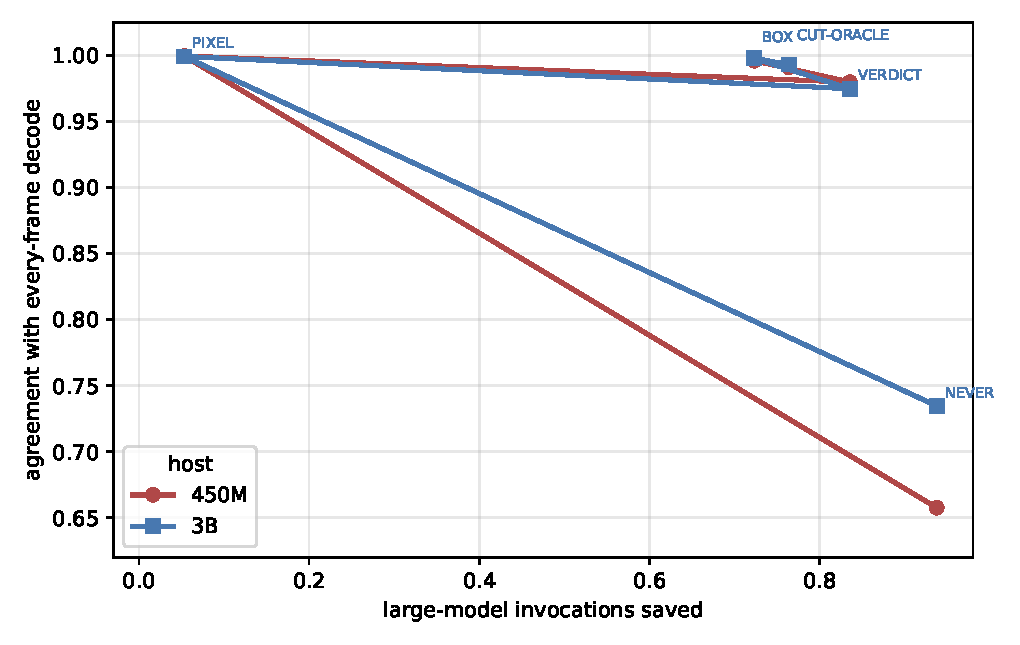
\includegraphics[width=0.82\linewidth]{gate-ladder.pdf}
\caption{Saved large-model invocations against mean social/caution agreement with every-frame decoding. Labels identify the registered gates; both points and paths come from pooled rung 2t artifacts.}
\label{fig:gates}
\end{figure}
\clearpage

\section{Related work}\label{sec:related}

\paragraph{Steering a frozen model from inside.} Adding a vector to a
model's residual stream to shift its behaviour is well established:
activation addition~\cite{turner2023} and representation
engineering~\cite{zou2023} derive steering directions from contrastive
prompts and inject them at one or more layers, and the wider control
literature has shown that the directions so found are often
low-dimensional and behaviourally legible. The bus of this paper is a
steering channel in that family with three differences that matter for
the result. The direction is not derived from a contrast but
\emph{trained through the host} toward an action, from a feature that
is itself the host's own state on the mode text; it is generated by a
hypernetwork~\cite{ha2016} rather than stored, so the same door serves
every mode phrasing including held-out ones; and it is injected on a
vision-language host with image tokens in the context, which is the
coexistence question \S\ref{sec:carriage} answers. The grounding result
--- a steering channel that leans on what the model sees rather than
overriding it --- has no direct precedent we are aware of, and the
blind-captain cell shows it is a property of the door's strength, not
of steering as such.

\paragraph{Soft prompts, prefixes, and adapters.} Prefix
tuning~\cite{li2021} and prompt tuning~\cite{lester2021} condition a
frozen model through learned embeddings in the prompt slot, and
LoRA~\cite{hu2021} through low-rank weight deltas. The program this
paper belongs to has compared those doors on the same hosts: a want
enters best where language enters, through a prefix, while a manner ---
a way of acting --- enters best through the bus~\cite{penov2026want}.
The modes here are manners in that sense, which is why the bus is the
channel under test rather than a prefix. The door recipe (a
conditioned latent bridge with receivers at depth fractions) is the
one that work established at 27B~\cite{penov2026act}, unchanged on the
language tower of each VL host.

\paragraph{Small models in front of large ones.} Vision-language agents
routinely place a cheap perception module ahead of a large model, and
tool-use frameworks let the large model call detectors as functions;
the difference here is the direction and the type of what crosses. The
lookout does not return a fact into the large model's context, where it
would be one more overridable token sequence; it sets a stance through
a channel the context cannot see, and the large model keeps the facts.
The compute result of \S\ref{sec:economics} is a behavioural analogue of
speculative decoding~\cite{leviathan2023,chen2023}: a cheap model
proposes that nothing changed and the expensive model is consulted only
on disagreement, with the difference that acceptance is not verified
and the cost of a wrong acceptance is one stale action. The gate's
failure mode is also the classical one from change detection and
event-based vision~\cite{gallego2020}: a threshold on raw pixel change
cannot separate camera noise from world change, and only a gate with a
semantic verdict can.

\paragraph{Sim-to-real for perception.} The rendered-world result of
\S\ref{sec:limits} touches the sim-to-real literature only at its
narrowest point --- whether a COCO-trained detector reads a rendered
person --- and finds the answer is entirely about the figure's shape
and texture rather than the renderer, in line with the domain-gap work
that motivates photorealistic and scanned assets. What is specific to
this architecture is that the doors' transfer, unlike the detector's,
is a training-recipe question rather than an asset question, and one
with a lever that also buys robustness.

\paragraph{Preregistration.} The registration protocol follows the
practice of preregistered studies in the empirical sciences ---
hypotheses, analyses, and decision rules fixed before data are seen ---
applied cell by cell to an engineering ladder, with the additional
discipline that each result names, without registering, the follow-ups
it makes obvious, so that the next cell is on record before its result
can shape it.


\section{Limitations and rung 3}\label{sec:limits}

The study's boundaries are stated before its transfer result, because
the transfer result is what tests them. Every number in
\S\ref{sec:carriage}--\S\ref{sec:economics} lives on COCO photographs
and, for the stream, on synthetic jitter episodes over those
photographs; the action space is three teacher-forced words; the doors
are one recipe on one language-tower depth prior, and the 27B is one
model family. Three door seeds is enough to read a majority and to
catch a headline that a replicate reverses --- it has, twice in this
program --- and not enough to estimate a seed distribution. The
registration protocol bounds what can be claimed but not what can be
imagined: a band written before a run is a commitment, not a proof
that the band was the right one, and the honest readings in
\S\ref{sec:price} and \S\ref{sec:safety} where the rule's verdict and
the numbers disagreed are the protocol working as intended rather than
a flaw in it.

Rung~3 is the boundary the robot cares about: render the world instead
of photographing it, and ask what transfers with nothing retrained. The
architectural stake was stated in advance. A door's packet is computed
from the mode phrasing's tap and never from the frame, so the doors
cannot fail to transfer \emph{by construction}; what is actually under
test is the two perceiving parts, the lookout's verdict and the
captain's own grounding, on rendered pixels. The scene is a floored
room with two to four coloured box obstacles, a camera with position
and yaw jitter, a jittered light, and a person placed within view; the
present rule is rung~1's, measured exactly instead of annotated ---
the person's segmentation mask must cover at least $5\%$ of the frame
--- and absent is the same drawn scene with the person removed; 100
present and 100 absent frames from one draw.

The first person was the simulator's stock capsule humanoid, at two
registered realism levels (stock appearance, then skin- and
clothing-coloured geoms). Table~\ref{tab:r3detector} is the reading:
zero person verdicts in 600 detector-level trials across three
detector sizes and both levels, zero false alarms, accuracy $0.50$ ---
a total sim gap. The mechanism is the useful part. This is not weak
person-signal under the threshold; it is a confident wrong parse. On
present frames the detector's best person confidence peaks at $0.03$
while the same frames yield \emph{sports ball} at $0.81$ (the head),
\emph{orange}, \emph{carrot}, \emph{knife}, and \emph{baseball bat}
(the capsule limbs). Capsule primitives never enter the person region
of COCO feature space, whatever their colour; the registered realism
ladder was aimed at the wrong axis. It is worth saying plainly for
anyone evaluating COCO detectors against primitive-based simulators:
zero false alarms and zero hits look like a conservative detector and
are total blindness. The captain, probed on the same capsule frames
under the caution text, discriminates at $0.267$ --- stopping for the
figure 27 points more often when it is present --- where every YOLO
scored exactly zero: MIXED by the registered band, and directionally
the captain out-sees the lookout in simulation.

One asset swap closes the gap. Rung~3b replaces the capsule with a
pinned photogrammetry scan of a clothed adult (HSR0081 from HSRD-100,
CC~BY~4.0), same rooms, cameras, lights, and draws; the render differs
from rung~3's only in the figure. The operating detector goes from
$0/100$ to $99/100$ present with zero false alarms, accuracy $0.995$.
The sim gap was the figure, entirely. Then the doors
(Table~\ref{tab:r3transfer}). At the 450M the unchanged COCO doors
travel at or above their photograph leans (s42 caution $1.00$ against
$0.78$ on COCO; social $0.50$ against $0.33$), grounding $0.00$
everywhere: for the small host the clean render is an easier frame than
a cluttered photograph. At the 3B the registered HOST-BLIND reading is
falsified by its own text arm --- on the same rendered frames the
caution text drives stop at $0.87$ and the social text greets at
$0.54$, so perception and language conditioning transfer perfectly ---
and what fails to transfer is the \emph{packet}: at s42 the packet
equals the habit on every mode, while the same doors lean $0.56$--$0.67$
on photographs. The failure is ordered by door strength, the study's
recurring axis: s42's weak doors die ($0.00$), s1042 sits at the
threshold ($0.23$), and s2042's near-perfect caution door travels at
full strength ($1.00$). The prediction that transfer would track the
host's perception was wrong in the informative direction. The door's
injection is frame-blind, but its \emph{effect} rides on
frame-conditioned residual state, and rendered frames put the 3B's
stream where only a strong door's direction still bites.

That turns the section into a prescription, and three registered cells
wrote it (Table~\ref{tab:domain}). Rung~3c doubled the steps: the
strength lever that had bought hostile survival for free moves the
domain gap and does not close it --- s42 caution $0.00\to0.31$, s1042
$0.23\to0.18$ --- so the gap lives partly in the door's
\emph{direction}, where in activation space its packet pushes, beyond
how hard. Rung~3d put 80 rendered frames into the training mix at the
registered step count: the mix closes the render gap outright ($0.95 /
0.86$) and pays for it in hostile robustness, s1042's caution ownership
under attack falling from $0.48$ to $0.125$ while calm conditioning
survives. The bus had a domain budget, and the detail said what it was
spent from: not the calm lean but the resistance margin. Rung~3e, the
synthesis, trained the mixed doors at twice the steps, and every band
passed with room --- renders $0.86 / 1.00$, calm packet shares retained
or improved, and hostile ownership $0.85$ against the registered door's
own $0.48$. The budget was a \emph{training} budget, not a bus-capacity
budget: the same 256-dimensional packet at the same dose holds two
domains and more margin than the single-domain door ever had. The lever
algebra closes. Mix buys direction, steps buy margin, and they compound
rather than compete; at the 3B the recommended door recipe is the
mixed domain at twice the steps, and there it dominates the registered
recipe on every axis measured.

Then the prescription was put to the other two hosts, and it did not
survive as written (rung~3f, Table~\ref{tab:scale}). At the 450M the
recipe \emph{trades}: it repairs the one seed whose registered doors did
not travel (caution on renders $0.07\to0.94$) and breaks the two that
did ($1.00\to0.36$ and $0.44$), halves one seed's calm caution on
photographs ($1.00\to0.50$) and inverts the explore packet --- DOMAIN
LOST by the registered band. What was a training budget at the 3B is a
capacity budget at the 450M: the same mix, steps, and bus cannot hold a
second domain in a smaller host's residual stream without dropping the
first. At the 27B the registered doors already travel unaided (two of
three seeds, caution leans $0.52 / 0.81 / 0.50$, the packet again above
the prompt on renders), and the recipe is mixed: it cures the
suggestible s2042 door of \S\ref{sec:price} (hostile ownership
$0.67\to1.17$, its grounding pulse $0.13\to0.07$, social awake on
renders), doubles the middle seed's margin ($0.92\to2.00$), and damages
seed~42, whose calm caution falls to $0.50$ on photographs at the 27B
exactly as at the 450M --- the same seed, the same number, at both new
hosts, with half of ``stop for people'' migrated into the pair's
constant door. The letter of the caution-lean band fails at the 27B for
a reason the table makes visible: the mixed-domain constant door is no
longer neutral on rendered person frames (it greets $0.85$ at one seed
and stops $0.94$ at another where the registered constant doors
proceed), so the lean's denominator moves while the packet's own stop
share saturates ($0.50 / 1.00 / 1.00$). The honest reading is that the
27B's mx2 packets travel at every seed and hold at two, and that mixing
the domains moves \emph{both} doors of the pair, which the 3B tolerated
and the other hosts did not. The prescription therefore comes with a
scale on it: at the onboard scale the recipe buys everything; at the
creature scale keep single-domain doors and repair gap seeds one at a
time; at the cortex scale the registered doors already travel and the
recipe is a per-seed cure with a per-seed cost. Two cells are named
and not registered: the seed-42 batch-order test, and a constant door
trained on photographs only while the mode door sees the mix.

What the transfer story does not yet cover is stated as plainly as
what it does. The rendered person is one identity in one static pose;
rung~3 tests transfer mechanics, not detector generality, which COCO
already established. Renders are not bit-reproducible across GPU or
driver changes on the same machine, which the registrations from rung~3f
onward handle by pinning scene identity and the detector reading
rather than pixel hashes. The gate of \S\ref{sec:economics} has not
been run on rendered episode streams or with a moving camera; the
27B has been put on renders but not yet through the gate; and the
three-word action space keeps every result here at the level of
behavioural modes, which is what the bus was built to carry and all it
has been shown to carry.

\par\medskip

\begin{center}
{\scriptsize
\setlength{\tabcolsep}{3pt}%
\begin{tabular}{llrrl}
\toprule
figure & level & person score & accuracy & what it sees \\
\midrule
capsule & l0 & 0.000 & 0.500 & -- \\
capsule & l1 & 0.000 & 0.500 & -- \\
mesh & mesh & 0.908 & 0.995 & -- \\
\bottomrule
\end{tabular}
}
\end{center}
\refstepcounter{table}
\noindent Table~\thetable: YOLO26s on capsule and photoscan renders. Person score is the mean person probability on present frames; descriptions are recorded detector outputs when available.
\label{tab:r3detector}
\par


\begin{center}
{\scriptsize
\setlength{\tabcolsep}{3pt}%
\begin{tabular}{lllrrr}
\toprule
host & recipe & mode & lean seeds & pooled & grounding \\
\midrule
450M & registered & social & 0.50/0.41/0.49 & 0.47 & 0.00 \\
450M & registered & caution & 1.00/0.07/1.00 & 0.69 & 0.00 \\
450M & registered & explore & 0.00/0.00/-0.50 & -0.17 & -- \\
3B & registered & social & 0.02/0.08/0.08 & 0.06 & 0.00 \\
3B & registered & caution & 0.00/0.23/1.00 & 0.41 & 0.00 \\
3B & registered & explore & 0.00/0.00/0.00 & 0.00 & -- \\
\bottomrule
\end{tabular}
}
\end{center}
\refstepcounter{table}
\noindent Table~\thetable: Unchanged registered doors on photoscan renders, seed order 42/1042/2042.
\label{tab:r3transfer}
\par


\begin{center}
{\scriptsize
\setlength{\tabcolsep}{3pt}%
\begin{tabular}{lrrr}
\toprule
recipe & render lean & calm packet & hostile ownership \\
\midrule
registered & 0.00/0.23/1.00 & 0.27/1.00/1.00 & 0.00/0.48/0.83 \\
x2 & 0.31/0.18 & 1.00 & 1.47 \\
mx & 0.95/0.86 & 0.97/0.90 & 0.35/0.12 \\
mx2 & 0.86/1.00 & 0.90/1.00 & 0.29/0.85 \\
\bottomrule
\end{tabular}
}
\end{center}
\refstepcounter{table}
\noindent Table~\thetable: The 3B caution domain budget by door recipe. Registered has seeds 42/1042/2042; x2, mx, and mx2 have seeds 42/1042. Capsule host-probe discrimination is 0.267.
\label{tab:domain}
\par


\begin{center}
{\scriptsize
\setlength{\tabcolsep}{3pt}%
\begin{tabular}{llrrrrr}
\toprule
host & recipe & render packet & render habit & render lean & calm packet & hostile ownership \\
\midrule
450M & registered & 1.00/0.07/1.00 & 0.00/0.00/0.00 & 1.00/0.07/1.00 & 1.00/1.00/1.00 & 0.97/1.33/1.00 \\
450M & mx2 & 0.50/1.00/1.00 & 0.14/0.06/0.56 & 0.36/0.94/0.44 & 0.50/0.97/1.00 & -5.00/1.12/1.18 \\
3B & registered & 0.00/0.23/1.00 & 0.00/0.00/0.00 & 0.00/0.23/1.00 & 0.27/1.00/1.00 & 0.00/0.48/0.83 \\
3B & mx2 & 1.00/1.00 & 0.14/0.00 & 0.86/1.00 & 0.90/1.00 & 0.29/0.85 \\
27B & registered & 0.55/0.82/0.50 & 0.03/0.01/0.00 & 0.52/0.81/0.50 & 1.00/1.00/1.00 & 1.17/0.92/0.67 \\
27B & mx2 & 0.50/1.00/1.00 & 0.07/0.03/0.94 & 0.43/0.97/0.06 & 0.50/1.00/0.97 & --/2.00/1.17 \\
\bottomrule
\end{tabular}
}
\end{center}
\refstepcounter{table}
\noindent Table~\thetable: Rung 3f: the mixed-domain 2x-step recipe against the registered doors at every host, caution mode, seed order 42/1042/2042 (3B mx2: 42/1042). Render columns are stop shares and lean on photoscan-render person frames; calm packet is the stop share on COCO person frames; ownership is against the hostile prompt at dose 1x.
\label{tab:scale}
\par

\clearpage

\section{Numbers appendix}
Every number in this scaffold is loaded from the JSON artifacts bundled under
\texttt{note18/artifacts/}. Seed columns read the per-seed files; pooled
columns read the no-suffix files. Registrations, admissibility bands, detector
rules, checkpoint hashes, frame-manifest hashes, and run metadata remain in
those artifacts. The source registrations and dated readings are in
\texttt{tracks/vision-mode/PLAN.md}; this renderer does not copy claims out of
prose or type numerical results into the manuscript.

\begin{thebibliography}{99}
\bibitem{penov2026act} F.~Penov. The Want Becomes the Act. Preprint,
2026. \url{https://github.com/kortexa-ai/legolm.basis}.
\bibitem{penov2026want} F.~Penov. The Want and the Way: One Door for
What, One Door for How. Preprint, 2026.
\url{https://github.com/kortexa-ai/legolm.basis}.
\bibitem{penov2026inside} F.~Penov. The Want That Lives Inside.
Preprint, 2026. \url{https://github.com/kortexa-ai/legolm.basis}.
\bibitem{lfm2026} Liquid AI. LFM2.5 model family. Model releases,
2025--2026. \url{https://huggingface.co/LiquidAI}.
\bibitem{qwen2026} Qwen Team. Qwen3.8 model family. Model releases,
2026. \url{https://huggingface.co/Qwen}.
\bibitem{turner2023} A.~Turner, L.~Thiergart, D.~Udell, G.~Leech,
U.~Mini, and M.~MacDiarmid. Activation addition: steering language
models without optimization. arXiv:2308.10248, 2023.
\bibitem{zou2023} A.~Zou et al. Representation engineering: a
top-down approach to AI transparency. arXiv:2310.01405, 2023.
\bibitem{ha2016} D.~Ha, A.~Dai, and Q.~V. Le. HyperNetworks.
arXiv:1609.09106, 2016.
\bibitem{li2021} X.~L. Li and P.~Liang. Prefix-tuning: optimizing
continuous prompts for generation. ACL, 2021.
\bibitem{lester2021} B.~Lester, R.~Al-Rfou, and N.~Constant. The power
of scale for parameter-efficient prompt tuning. EMNLP, 2021.
\bibitem{hu2021} E.~J. Hu et al. LoRA: low-rank adaptation of large
language models. arXiv:2106.09685, 2021.
\bibitem{leviathan2023} Y.~Leviathan, M.~Kalman, and Y.~Matias. Fast
inference from transformers via speculative decoding. ICML, 2023.
\bibitem{chen2023} C.~Chen, S.~Borgeaud, G.~Irving, J.-B. Lespiau,
L.~Sifre, and J.~Jumper. Accelerating large language model decoding
with speculative sampling. arXiv:2302.01318, 2023.
\bibitem{gallego2020} G.~Gallego et al. Event-based vision: a survey.
IEEE TPAMI, 2020.
\end{thebibliography}

\end{document}
